%TC:ignore
\chapter{Further Results}
\label{appendix:results}

\section{Input images}

\begin{figure}[H]
    \centering
    \begin{subfigure}[t]{0.3\textwidth}
        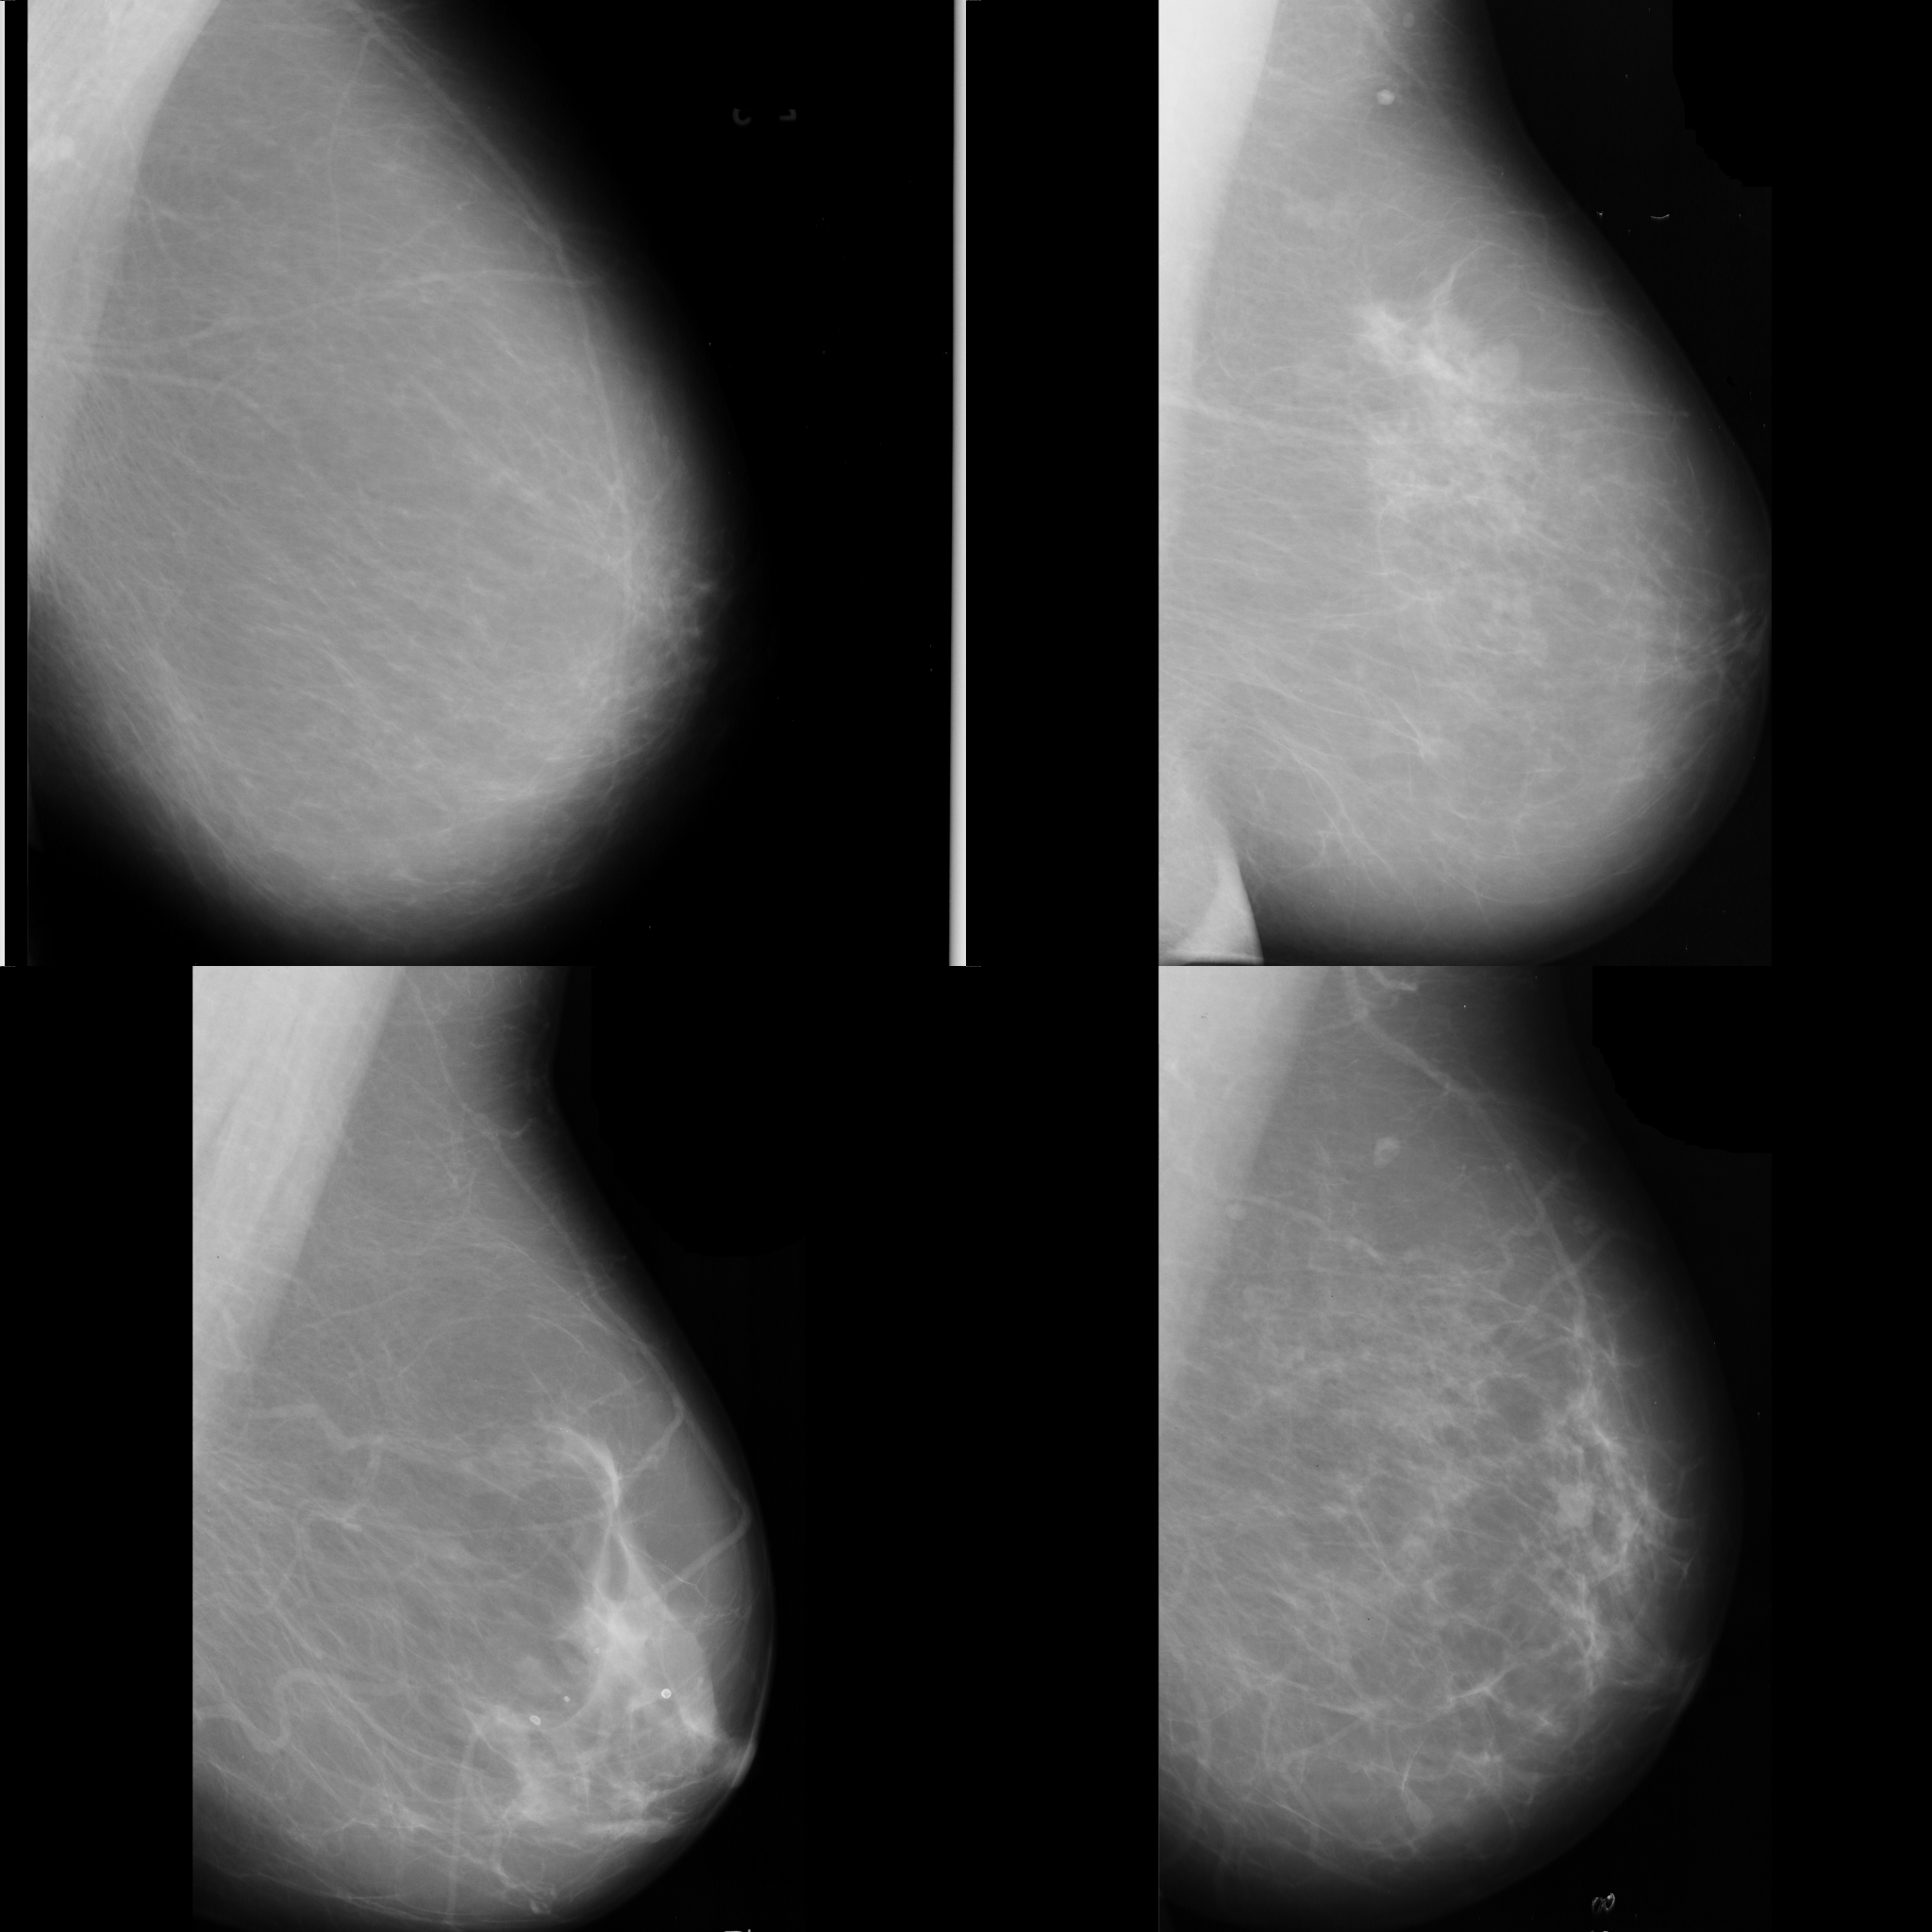
\includegraphics[width=\textwidth]{Appendix5/sample1/big_scan.png}
        \caption{BI-RADS I classification.}
        \label{fig:app-sample1-input}
    \end{subfigure}
    ~ %add desired spacing between images, e. g. ~, \quad, \qquad, \hfill etc.
      %(or a blank line to force the subfigure onto a new line)
    \begin{subfigure}[t]{0.3\textwidth}
        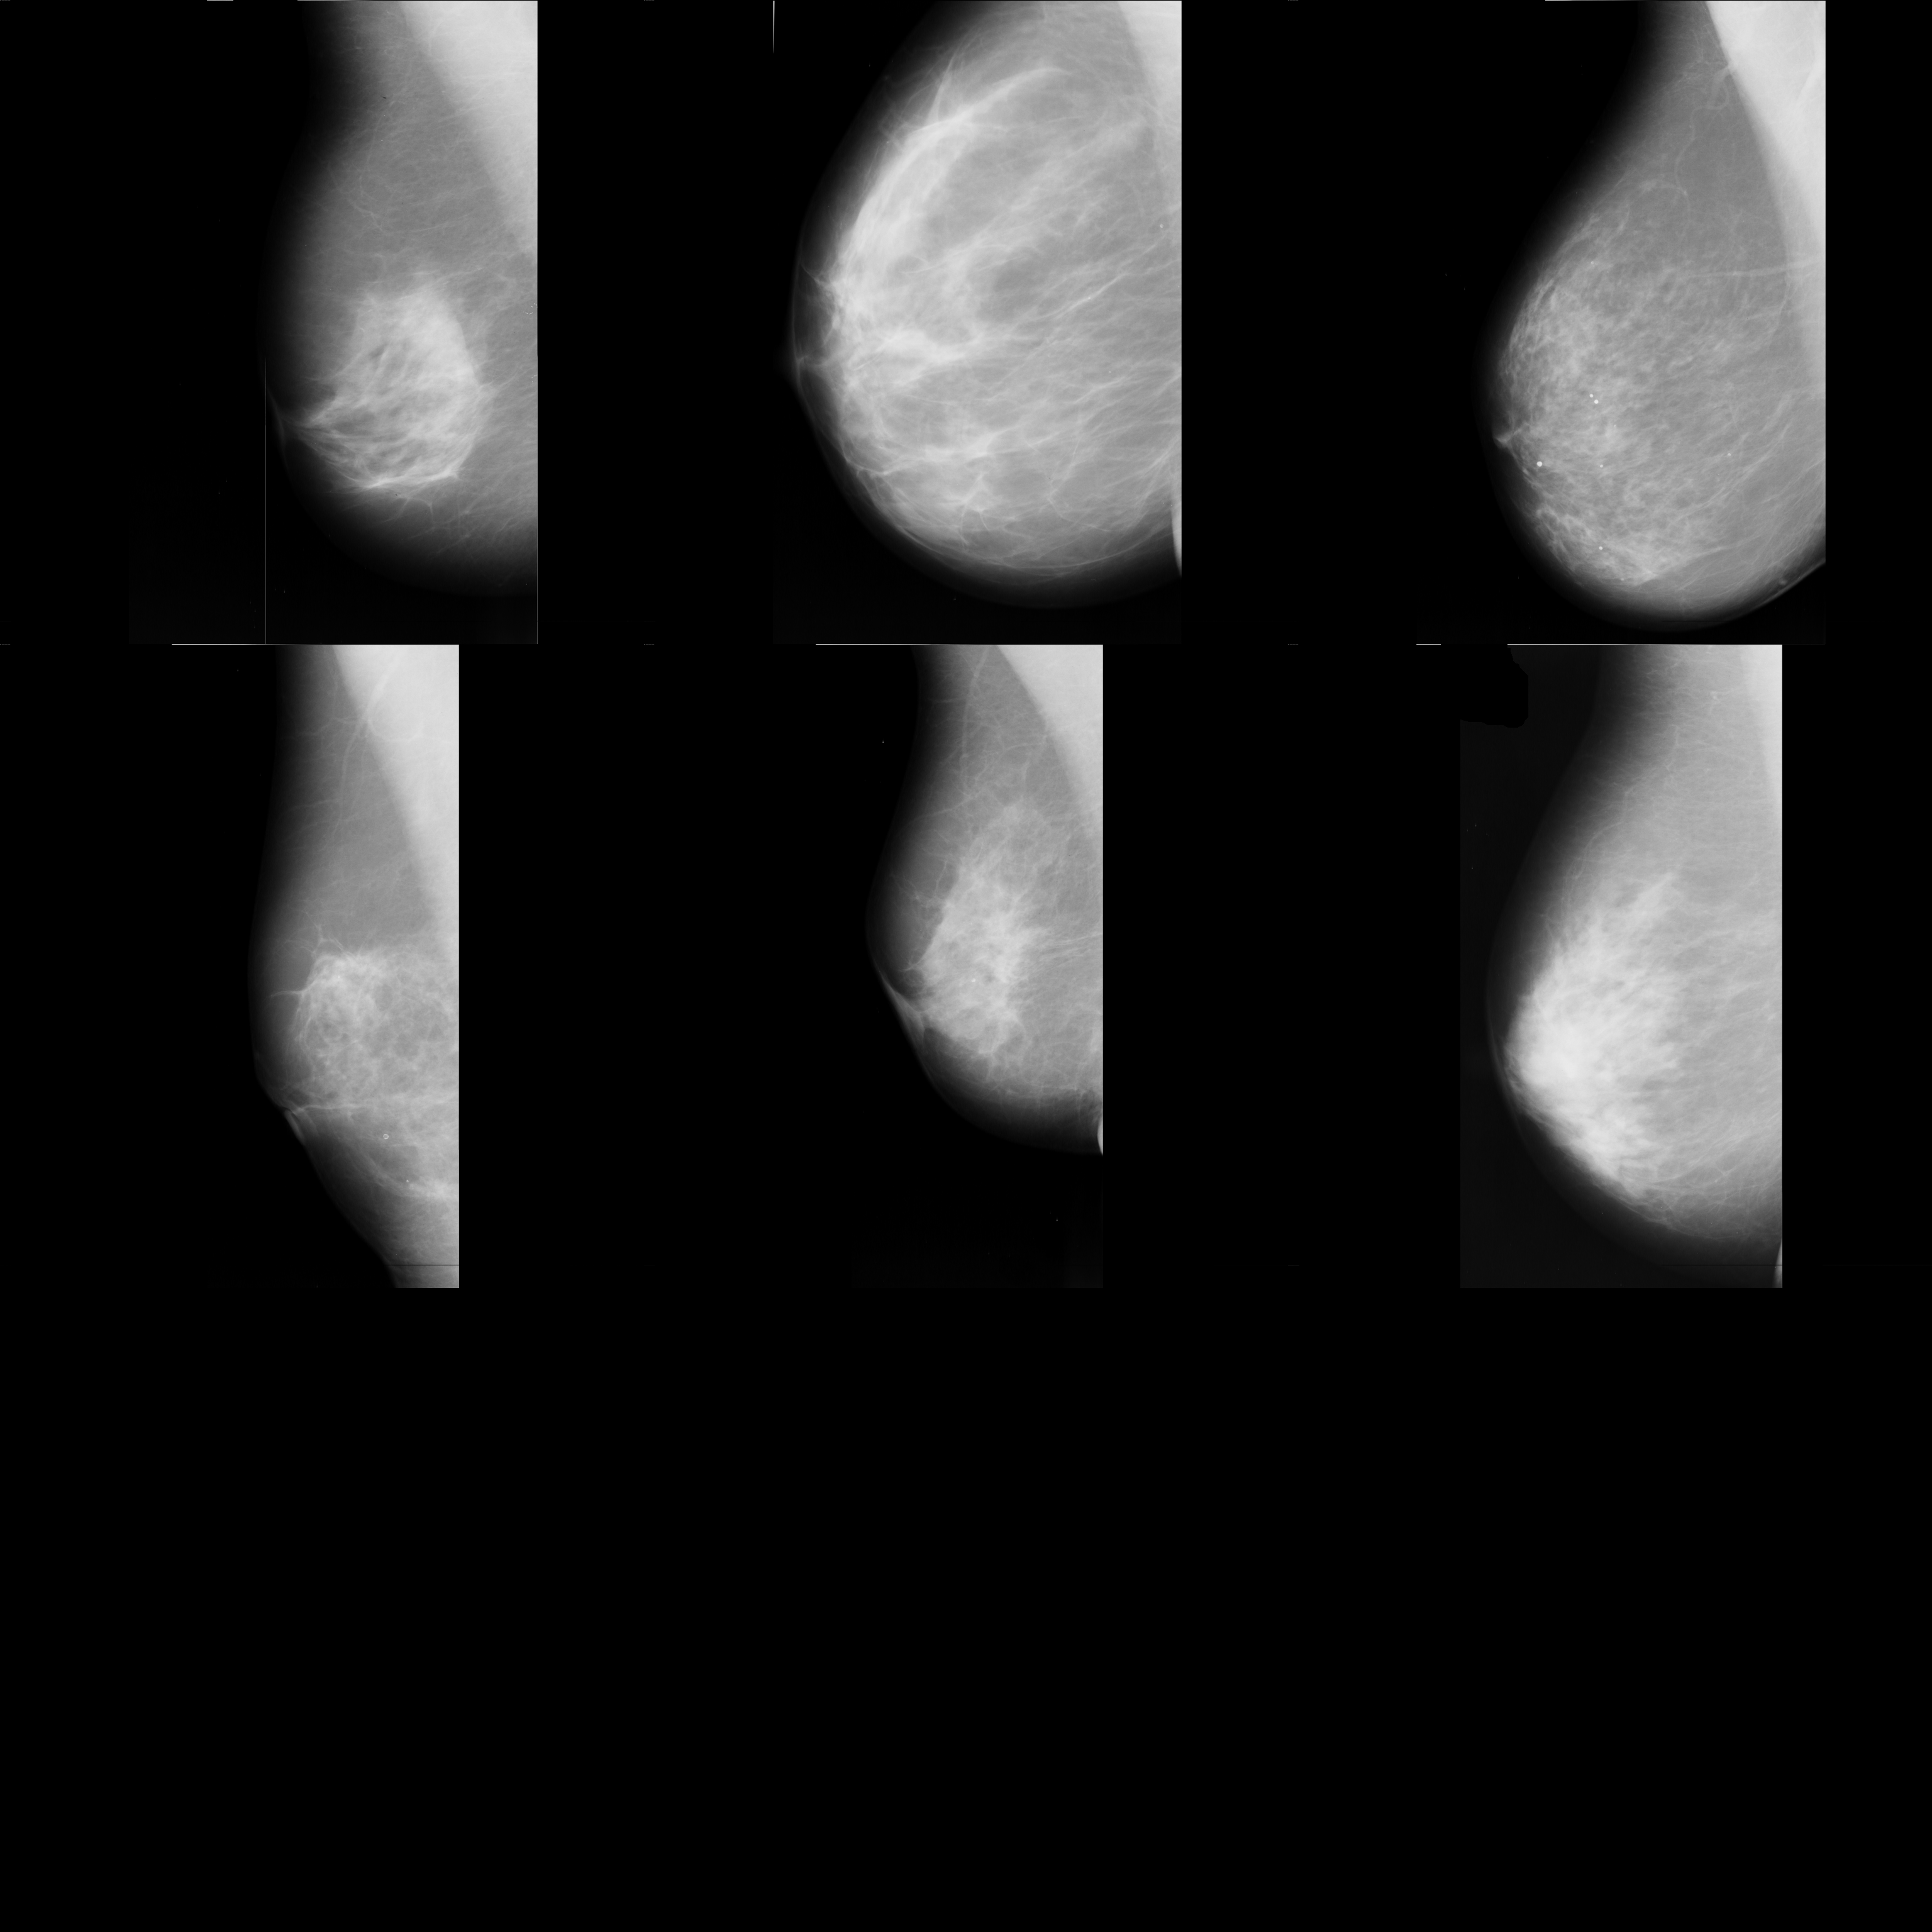
\includegraphics[width=\textwidth]{Appendix5/sample2/big_scan_sample2.png}
        \caption{BI-RADS II classification.}
        \label{fig:app-sample2-input}
    \end{subfigure}

    \begin{subfigure}[t]{0.3\textwidth}
      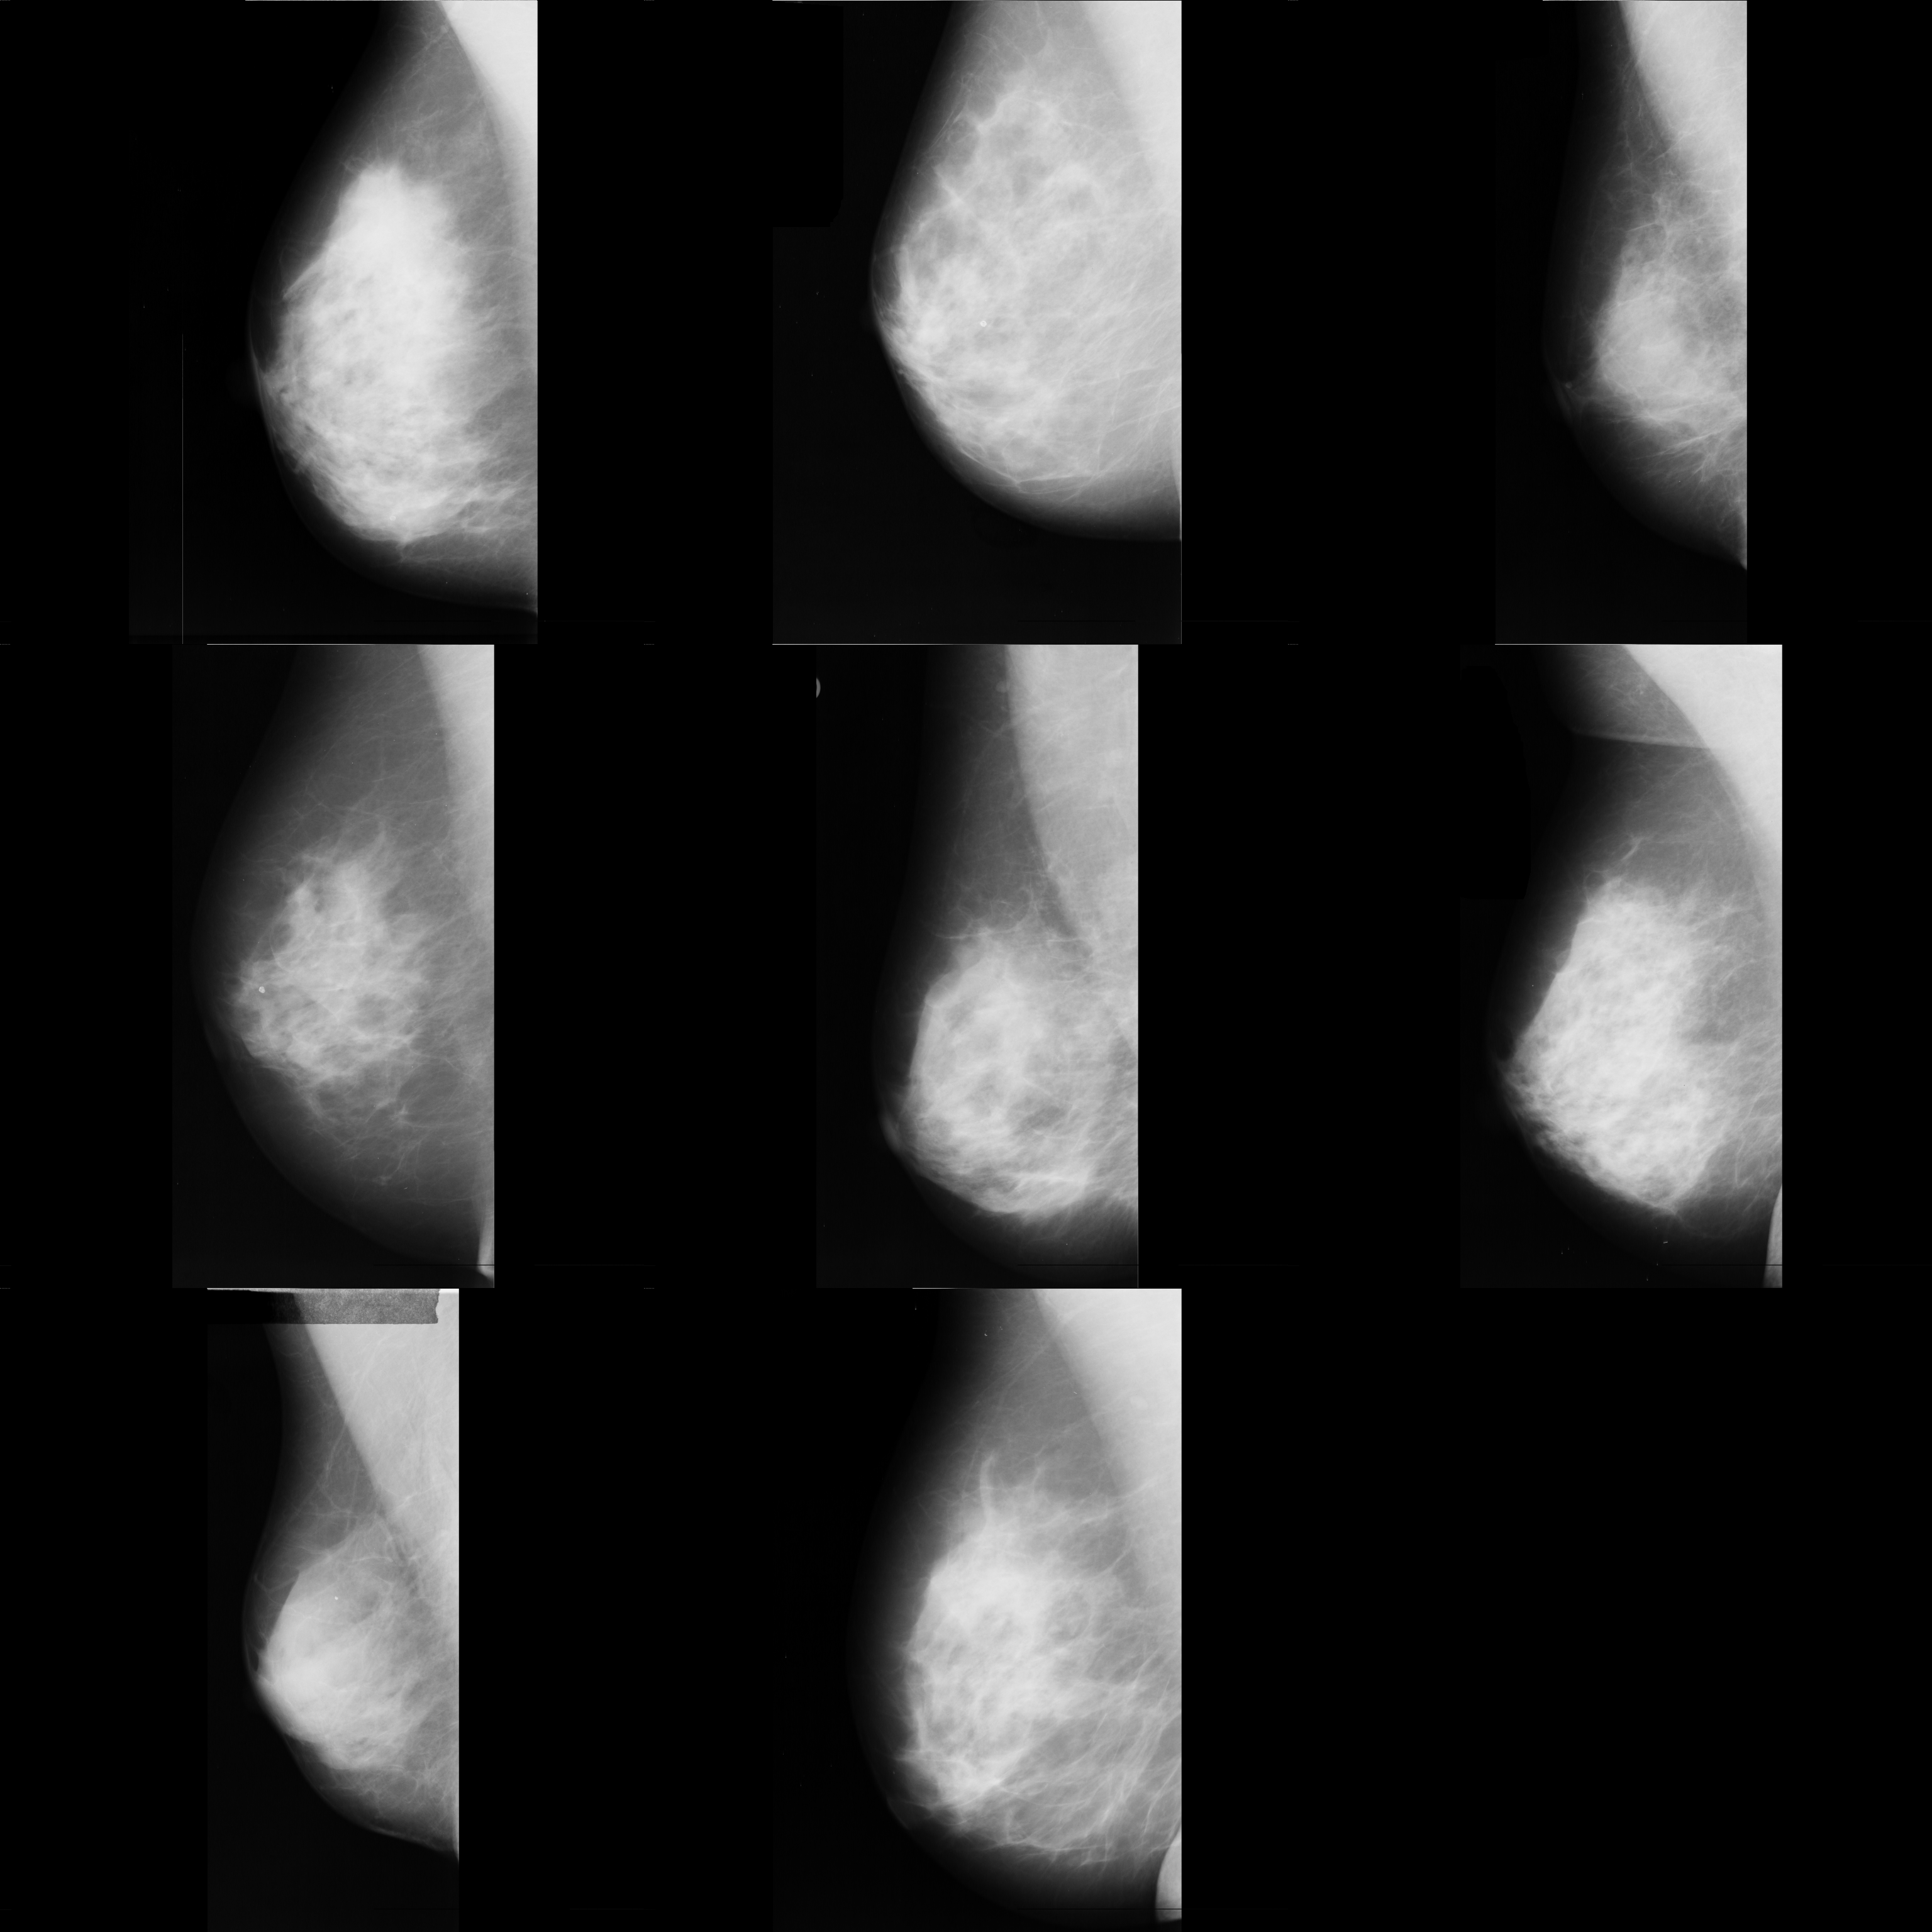
\includegraphics[width=\textwidth]{Appendix5/sample3/big_scan_sample3.png}
      \caption{BI-RADS III classification.}
      \label{fig:app-sample3-input}
    \end{subfigure}
    \begin{subfigure}[t]{0.3\textwidth}
      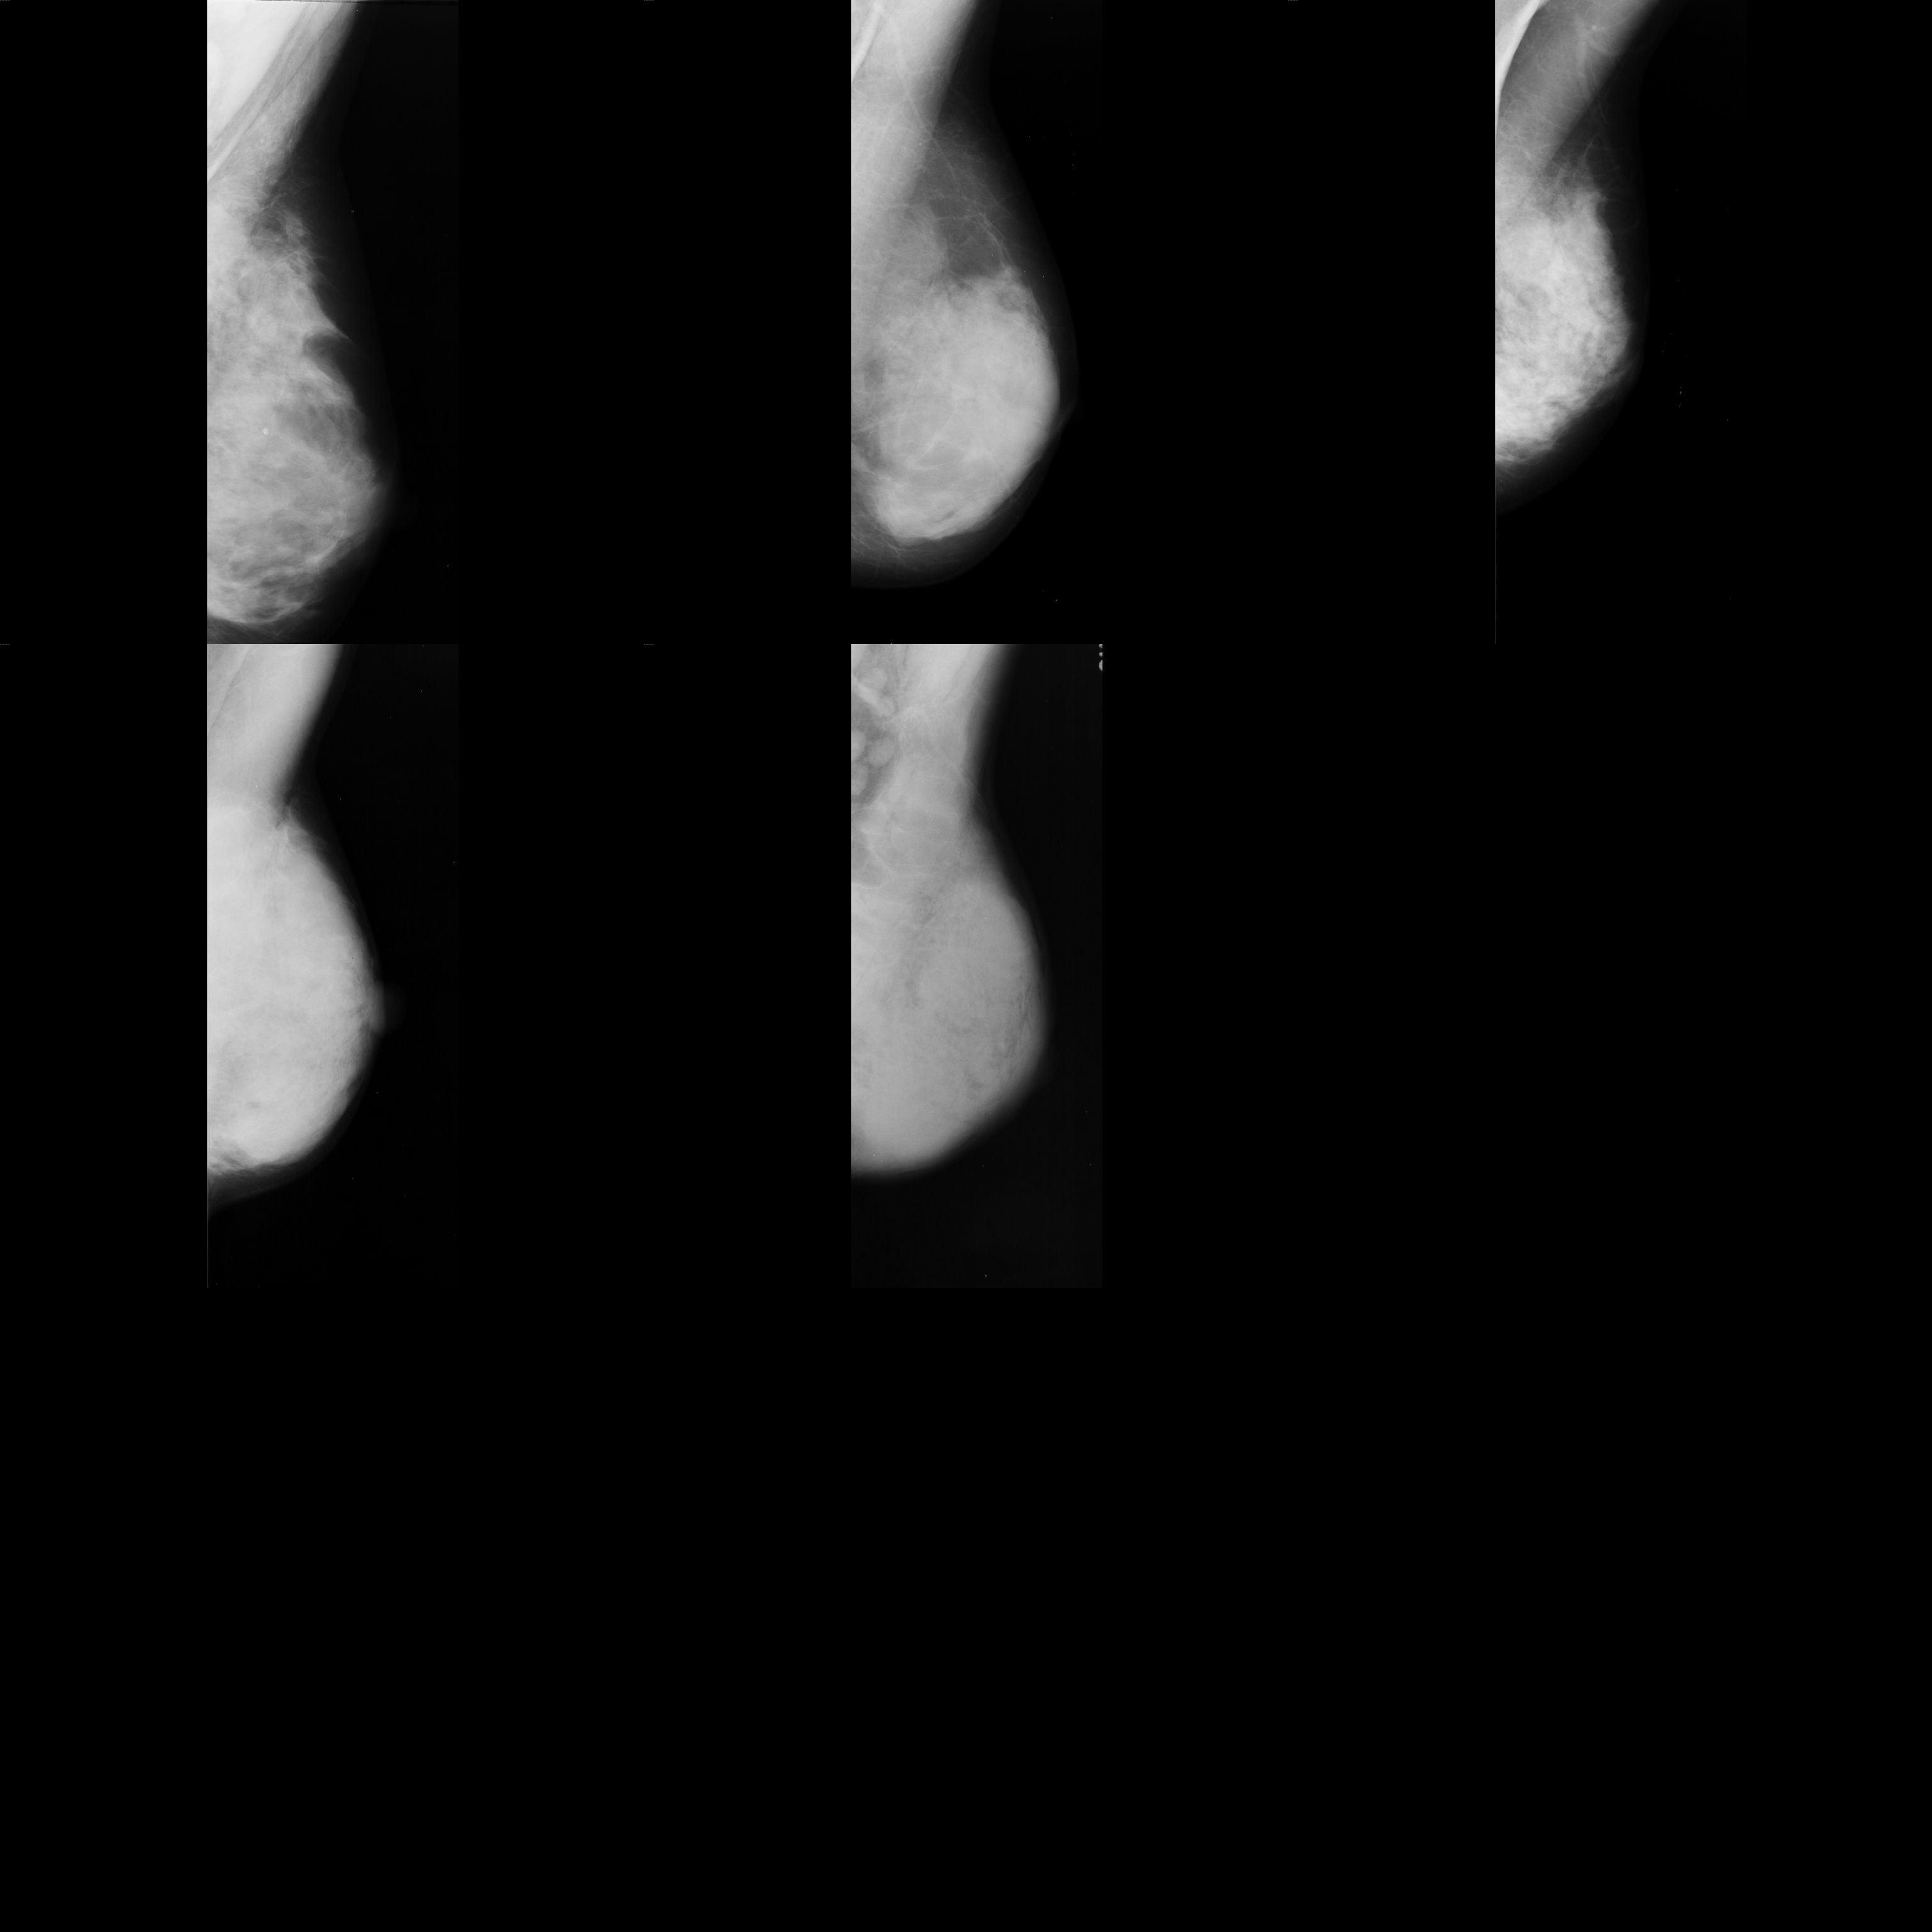
\includegraphics[width=\textwidth]{Appendix5/sample4/big_scan_sample4.png}
      \caption{BI-RADS IV classification.}
      \label{fig:app-sample4-input}
    \end{subfigure}
    \label{fig:all-input-imgs}
\end{figure}

\newpage
\section{Shannon Entropy}
\label{sec:app-shannon}

\noindent \textbf{Sample 1 - BI-RADS I}

Input image: Figure \ref{fig:app-sample1-input}

\begin{figure}[H]
    \centering
    \begin{subfigure}[t]{0.3\textwidth}
        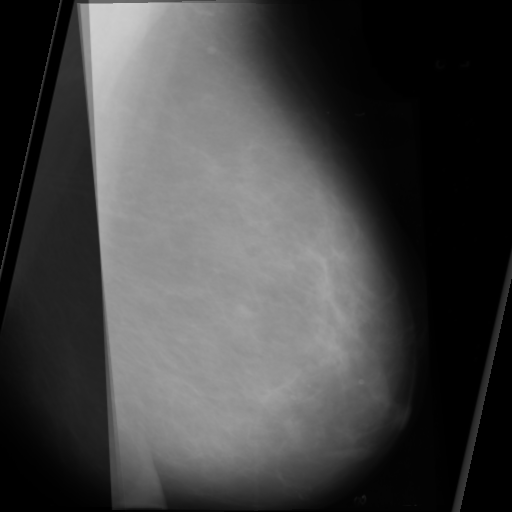
\includegraphics[width=\textwidth]{Appendix5/sample1/shannon/s-5-final.png}
        \caption{5 Shannon Entropy iterations.}
        \label{fig:app-5-shannon-sample1}
    \end{subfigure} \hfill
    ~ %add desired spacing between images, e. g. ~, \quad, \qquad, \hfill etc.
      %(or a blank line to force the subfigure onto a new line)
    \begin{subfigure}[t]{0.3\textwidth}
        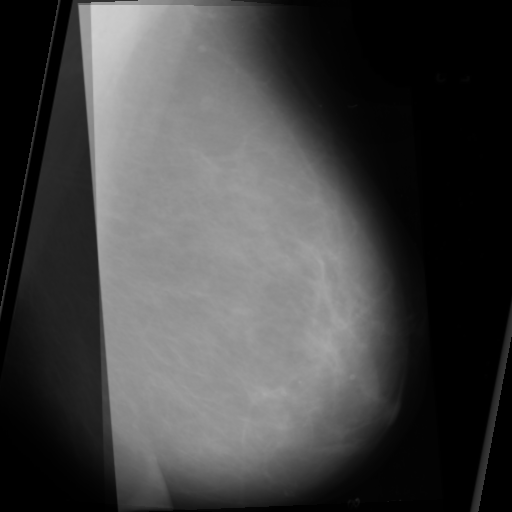
\includegraphics[width=\textwidth]{Appendix5/sample1/shannon/s-10-final.png}
        \caption{10 Shannon Entropy iterations.}
        \label{fig:app-10-shannon-sample1}
    \end{subfigure} \hfill
    \begin{subfigure}[t]{0.3\textwidth}
      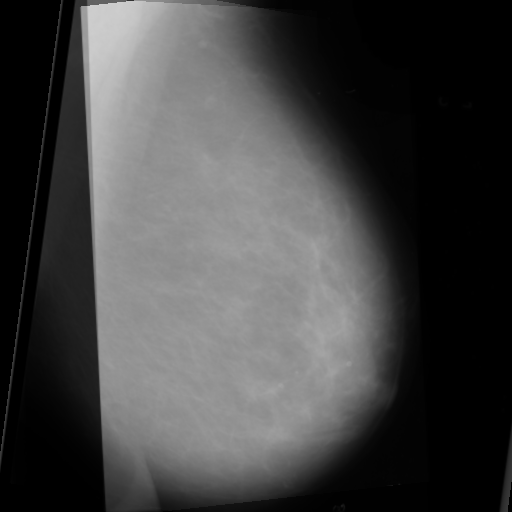
\includegraphics[width=\textwidth]{Appendix5/sample1/shannon/shannon-20.png}
      \caption{20 Shannon Entropy iterations.}
      \label{fig:app-20-shannon-sample1}
    \end{subfigure}
\end{figure}

\begin{table}[H]
  \begin{center}
    \pgfplotstabletypeset[col sep=comma,
        columns={Iteration,Entropy, Iteration, Entropy},columns/Entropy/.style={precision=6},
        every head row/.style={before row=\toprule,after row=\midrule},
        every last row/.style={after row=\bottomrule},
        display columns/0/.style={
            select equal part entry of={0}{2},
            string type,
            column name={Iteration (1/2)},
        },
        display columns/1/.style={
            select equal part entry of={0}{2},
            string type,
            column name={Entropy (1/2)},
        },
        display columns/2/.style={select equal part entry of={1}{2},string type}, column name={Iteration (2/2)},
        display columns/3/.style={select equal part entry of={1}{2},string type, column name={Entropy (2/2)}},
        ]{Appendix5/sample1/shannon/shannon-20.csv}
    \caption{Shannon entropy on Sample 1}
    \label{table:app-shannon-entropy-1}
  \end{center}
\end{table}


\newpage \noindent \textbf{Sample 2 - BI-RADS II}

Input image: Figure \ref{fig:app-sample2-input}

\begin{figure}[H]
    \centering
    \begin{subfigure}[t]{0.3\textwidth}
        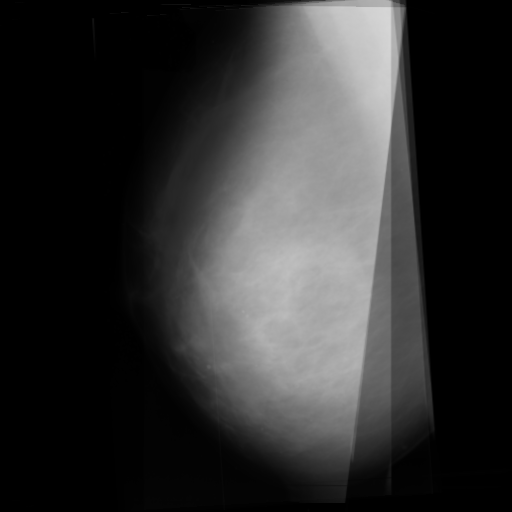
\includegraphics[width=\textwidth]{Appendix5/sample2/shannon/5_scan.png}
        \caption{5 Shannon Entropy iterations.}
        \label{fig:app-5-shannon-sample2}
    \end{subfigure} \hfill
    ~ %add desired spacing between images, e. g. ~, \quad, \qquad, \hfill etc.
      %(or a blank line to force the subfigure onto a new line)
    \begin{subfigure}[t]{0.3\textwidth}
        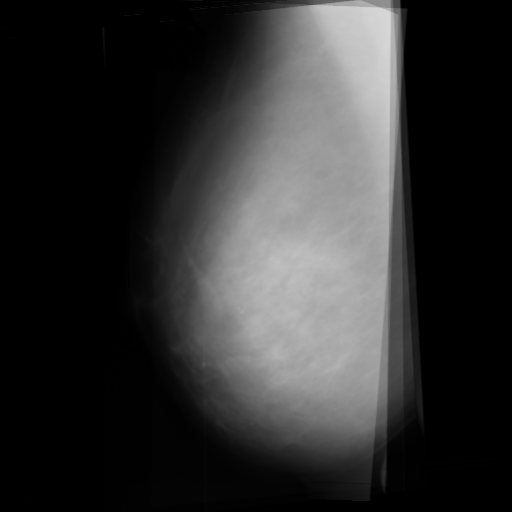
\includegraphics[width=\textwidth]{Appendix5/sample2/shannon/10_scan.png}
        \caption{10 Shannon Entropy iterations.}
        \label{fig:app-10-shannon-sample2}
    \end{subfigure} \hfill
    \begin{subfigure}[t]{0.3\textwidth}
      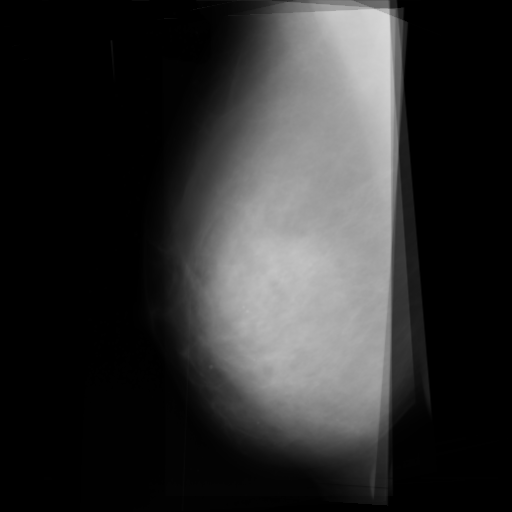
\includegraphics[width=\textwidth]{Appendix5/sample2/shannon/20_scan.png}
      \caption{20 Shannon Entropy iterations.}
      \label{fig:app-20-shannon-sample2}
    \end{subfigure}
\end{figure}

\begin{table}[H]
  \begin{center}
    \pgfplotstabletypeset[col sep=comma,
        columns={Iteration,Entropy, Iteration, Entropy},columns/Entropy/.style={precision=6},
        every head row/.style={before row=\toprule,after row=\midrule},
        every last row/.style={after row=\bottomrule},
        display columns/0/.style={
            select equal part entry of={0}{2},
            string type,
            column name={Iteration (1/2)},
        },
        display columns/1/.style={
            select equal part entry of={0}{2},
            string type,
            column name={Entropy (1/2)},
        },
        display columns/2/.style={select equal part entry of={1}{2},string type}, column name={Iteration (2/2)},
        display columns/3/.style={select equal part entry of={1}{2},string type, column name={Entropy (2/2)}},
        ]{Appendix5/sample2/shannon/shannon_entropy.csv}
    \caption{Shannon Entropy on Sample 2}
    \label{table:app-shannon-entropy-2}
  \end{center}
\end{table}

\newpage
\noindent \textbf{Sample 3 - BI-RADS III}

Input image: Figure \ref{fig:app-sample3-input}

\begin{figure}[H]
    \centering
    \begin{subfigure}[t]{0.3\textwidth}
        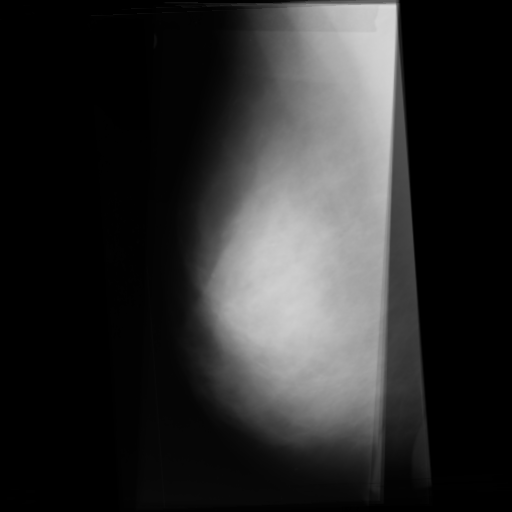
\includegraphics[width=\textwidth]{Appendix5/sample3/shannon/5_shannon.png}
        \caption{5 Shannon Entropy iterations.}
        \label{fig:app-5-shannon-sample3}
    \end{subfigure} \hfill
    ~ %add desired spacing between images, e. g. ~, \quad, \qquad, \hfill etc.
      %(or a blank line to force the subfigure onto a new line)
    \begin{subfigure}[t]{0.3\textwidth}
        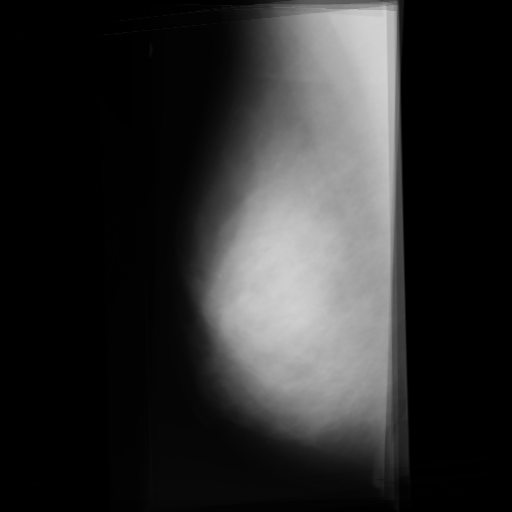
\includegraphics[width=\textwidth]{Appendix5/sample3/shannon/10_shannon.png}
        \caption{10 Shannon Entropy iterations.}
        \label{fig:app-10-shannon-sample3}
    \end{subfigure} \hfill
    \begin{subfigure}[t]{0.3\textwidth}
      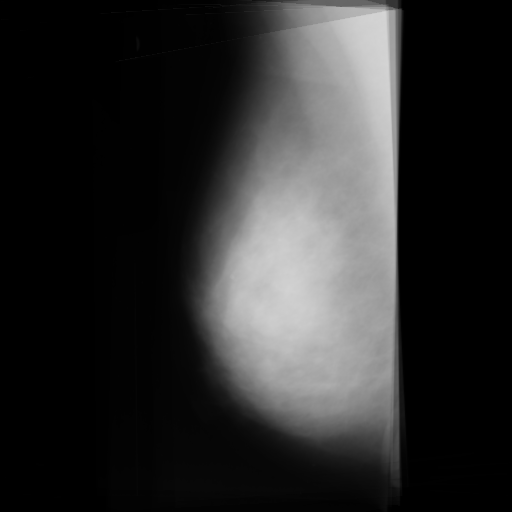
\includegraphics[width=\textwidth]{Appendix5/sample3/shannon/20_shannon.png}
      \caption{20 Shannon Entropy iterations.}
      \label{fig:app-20-shannon-sample3}
    \end{subfigure}
\end{figure}

\begin{table}[H]
  \begin{center}
    \pgfplotstabletypeset[col sep=comma,
        columns={Iteration,Entropy, Iteration, Entropy},columns/Entropy/.style={precision=6},
        every head row/.style={before row=\toprule,after row=\midrule},
        every last row/.style={after row=\bottomrule},
        display columns/0/.style={
            select equal part entry of={0}{2},
            string type,
            column name={Iteration (1/2)},
        },
        display columns/1/.style={
            select equal part entry of={0}{2},
            string type,
            column name={Entropy (1/2)},
        },
        display columns/2/.style={select equal part entry of={1}{2},string type}, column name={Iteration (2/2)},
        display columns/3/.style={select equal part entry of={1}{2},string type, column name={Entropy (2/2)}},
        ]{Appendix5/sample3/shannon/shannon.csv}
    \caption{Shannon Entropy on Sample 3}
    \label{table:app-shannon-entropy-3}
  \end{center}
\end{table}

\newpage \noindent \textbf{Sample 4 - BI-RADS IV}

Input image: Figure \ref{fig:app-sample4-input}

\begin{figure}[H]
    \centering
    \begin{subfigure}[t]{0.3\textwidth}
        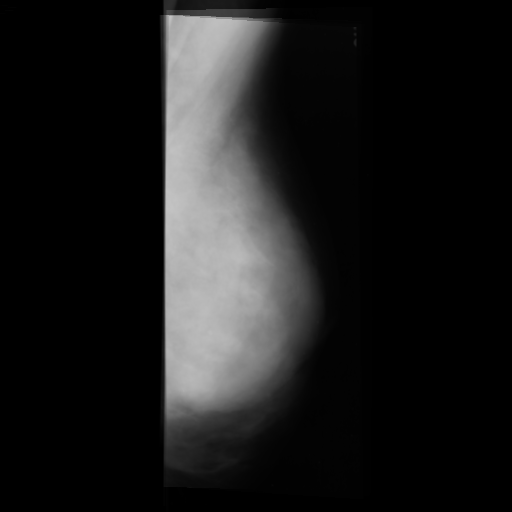
\includegraphics[width=\textwidth]{Appendix5/sample4/shannon/shannon_5.png}
        \caption{5 Shannon Entropy iterations.}
        \label{fig:app-5-shannon-sample4}
    \end{subfigure} \hfill
    ~ %add desired spacing between images, e. g. ~, \quad, \qquad, \hfill etc.
      %(or a blank line to force the subfigure onto a new line)
    \begin{subfigure}[t]{0.3\textwidth}
        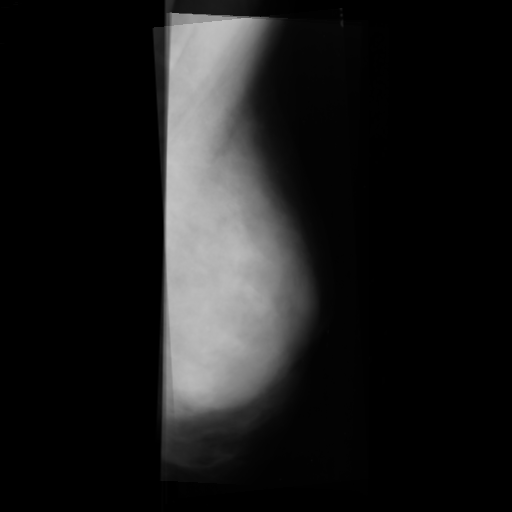
\includegraphics[width=\textwidth]{Appendix5/sample4/shannon/shannon_10.png}
        \caption{10 Shannon Entropy iterations.}
        \label{fig:app-10-shannon-sample4}
    \end{subfigure} \hfill
    \begin{subfigure}[t]{0.3\textwidth}
      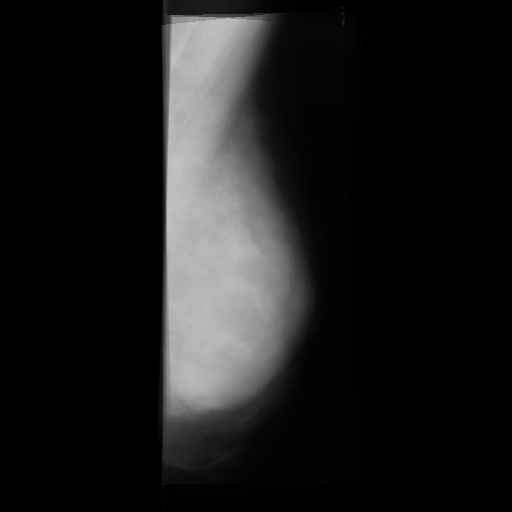
\includegraphics[width=\textwidth]{Appendix5/sample4/shannon/shannon_20.png}
      \caption{20 Shannon Entropy iterations.}
      \label{fig:app-20-shannon-sample4}
    \end{subfigure}
\end{figure}

\begin{table}[H]
  \begin{center}
    \pgfplotstabletypeset[col sep=comma,
        columns={Iteration,Entropy, Iteration, Entropy},columns/Entropy/.style={precision=6},
        every head row/.style={before row=\toprule,after row=\midrule},
        every last row/.style={after row=\bottomrule},
        display columns/0/.style={
            select equal part entry of={0}{2},
            string type,
            column name={Iteration (1/2)},
        },
        display columns/1/.style={
            select equal part entry of={0}{2},
            string type,
            column name={Entropy (1/2)},
        },
        display columns/2/.style={select equal part entry of={1}{2},string type}, column name={Iteration (2/2)},
        display columns/3/.style={select equal part entry of={1}{2},string type, column name={Entropy (2/2)}},
        ]{Appendix5/sample4/shannon/shannon.csv}
    \caption{Shannon Entropy on Sample 4}
    \label{table:app-shannon-entropy-4}
  \end{center}
\end{table}

\newpage
\section{Non-Probabilistic Entropy}

\noindent \textbf{Sample 1 - BI-RADS I}

Input image: Figure \ref{fig:app-sample1-input}

\begin{figure}[H]
    \centering
    \begin{subfigure}[t]{0.3\textwidth}
        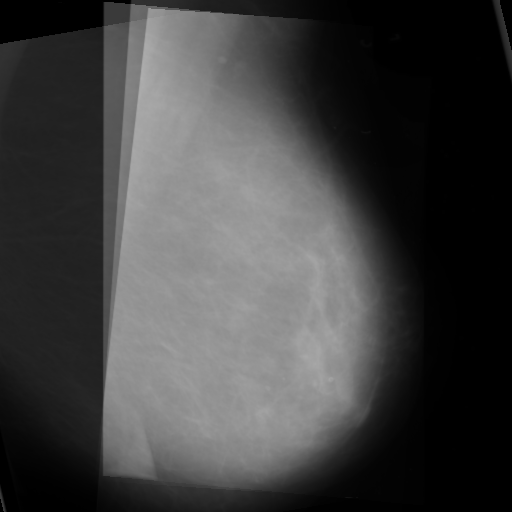
\includegraphics[width=\textwidth]{Appendix5/sample1/nonProb/nonProb-5.png}
        \caption{5 Non-Probabilistic Entropy iterations.}
        \label{fig:app-5-nonProb-sample1}
    \end{subfigure} \hfill
    ~ %add desired spacing between images, e. g. ~, \quad, \qquad, \hfill etc.
      %(or a blank line to force the subfigure onto a new line)
    \begin{subfigure}[t]{0.3\textwidth}
      \includegraphics[width=\textwidth]{Appendix5/sample1/nonProb/nonProb10.png}
      \caption{10 Non-Probabilistic Entropy iterations.}
      \label{fig:app-10-nonProb-sample1}
    \end{subfigure} \hfill
    \begin{subfigure}[t]{0.3\textwidth}
      \includegraphics[width=\textwidth]{Appendix5/sample1/nonProb/nonProb20.png}
      \caption{20 Non-Probabilistic Entropy iterations.}
      \label{fig:app-20-nonProb-sample1}
    \end{subfigure}
\end{figure}

\begin{table}[H]
  \begin{center}
    \pgfplotstabletypeset[col sep=comma,
        columns={Iteration,Entropy, Iteration, Entropy},columns/Entropy/.style={precision=6},
        every head row/.style={before row=\toprule,after row=\midrule},
        every last row/.style={after row=\bottomrule},
        display columns/0/.style={
            select equal part entry of={0}{2},
            string type,
            column name={Iteration (1/2)},
        },
        display columns/1/.style={
            select equal part entry of={0}{2},
            string type,
            column name={Entropy (1/2)},
        },
        display columns/2/.style={select equal part entry of={1}{2},string type}, column name={Iteration (2/2)},
        display columns/3/.style={select equal part entry of={1}{2},string type, column name={Entropy (2/2)}},
        ]{Appendix5/sample1/nonProb/nonProb20.csv}
    \caption{Non-Probabilistic Entropy on Sample 1}
    \label{table:app-nonProb-entropy-1}
  \end{center}
\end{table}

\newpage \noindent \textbf{Sample 2 - BI-RADS II}

Input image: Figure \ref{fig:app-sample2-input}

\begin{figure}[H]
    \centering
    \begin{subfigure}[t]{0.3\textwidth}
        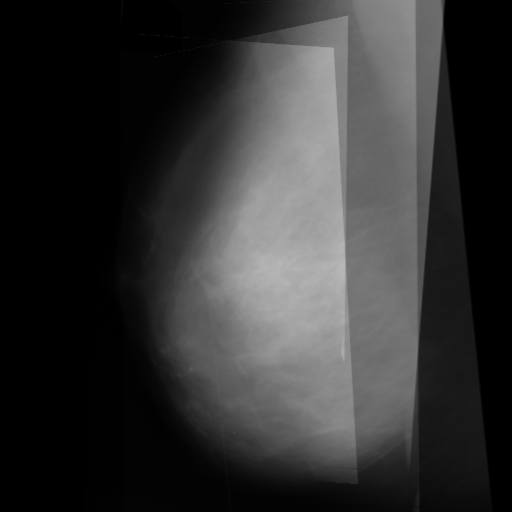
\includegraphics[width=\textwidth]{Appendix5/sample2/nonProb/5_scan.png}
        \caption{5 Non-Probabilistic Entropy iterations.}
        \label{fig:app-5-nonProb-sample2}
    \end{subfigure} \hfill
    ~ %add desired spacing between images, e. g. ~, \quad, \qquad, \hfill etc.
      %(or a blank line to force the subfigure onto a new line)
    \begin{subfigure}[t]{0.3\textwidth}
      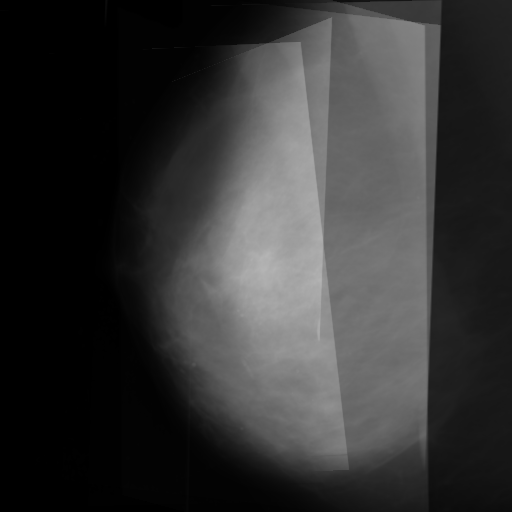
\includegraphics[width=\textwidth]{Appendix5/sample2/nonProb/10_scan.png}
      \caption{10 Non-Probabilistic Entropy iterations.}
      \label{fig:app-10-nonProb-sample2}
    \end{subfigure} \hfill
    \begin{subfigure}[t]{0.3\textwidth}
      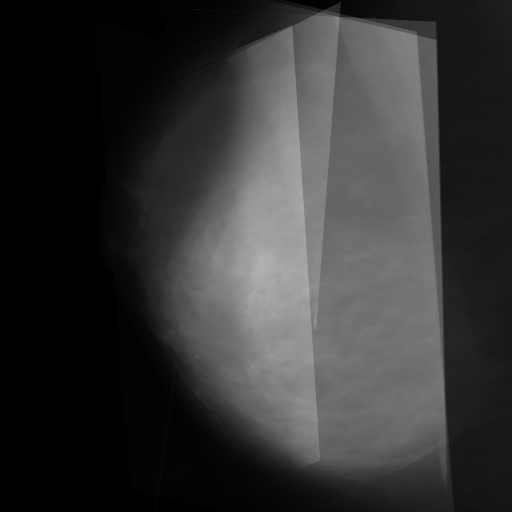
\includegraphics[width=\textwidth]{Appendix5/sample2/nonProb/20_scan.png}
      \caption{20 Non-Probabilistic Entropy iterations.}
      \label{fig:app-20-nonProb-sample2}
    \end{subfigure}
\end{figure}

\begin{table}[H]
  \begin{center}
    \pgfplotstabletypeset[col sep=comma,
        columns={Iteration,Entropy, Iteration, Entropy},columns/Entropy/.style={precision=6},
        every head row/.style={before row=\toprule,after row=\midrule},
        every last row/.style={after row=\bottomrule},
        display columns/0/.style={
            select equal part entry of={0}{2},
            string type,
            column name={Iteration (1/2)},
        },
        display columns/1/.style={
            select equal part entry of={0}{2},
            string type,
            column name={Entropy (1/2)},
        },
        display columns/2/.style={select equal part entry of={1}{2},string type}, column name={Iteration (2/2)},
        display columns/3/.style={select equal part entry of={1}{2},string type, column name={Entropy (2/2)}},
        ]{Appendix5/sample2/nonProb/nonProb.csv}
    \caption{Non-Probabilistic Entropy on Sample 2}
    \label{table:app-nonProb-entropy-2}
  \end{center}
\end{table}

\newpage
\noindent \textbf{Sample 3 - BI-RADS III}

Input image: Figure \ref{fig:app-sample3-input}

\begin{figure}[H]
    \centering
    \begin{subfigure}[t]{0.3\textwidth}
        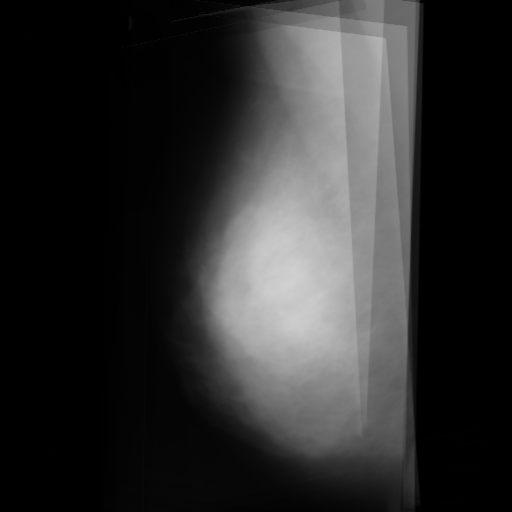
\includegraphics[width=\textwidth]{Appendix5/sample3/nonProb/5_scan.png}
        \caption{5 Non-Probabilistic Entropy iterations.}
        \label{fig:app-5-nonProb-sample3}
    \end{subfigure} \hfill
    ~ %add desired spacing between images, e. g. ~, \quad, \qquad, \hfill etc.
      %(or a blank line to force the subfigure onto a new line)
    \begin{subfigure}[t]{0.3\textwidth}
      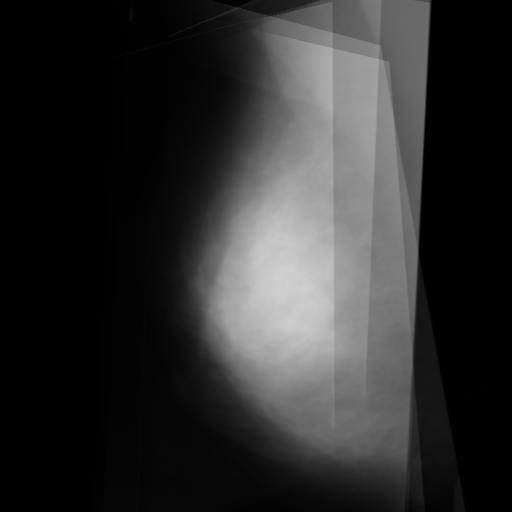
\includegraphics[width=\textwidth]{Appendix5/sample3/nonProb/10_scan.png}
      \caption{10 Non-Probabilistic Entropy iterations.}
      \label{fig:app-10-nonProb-sample3}
    \end{subfigure} \hfill
    \begin{subfigure}[t]{0.3\textwidth}
      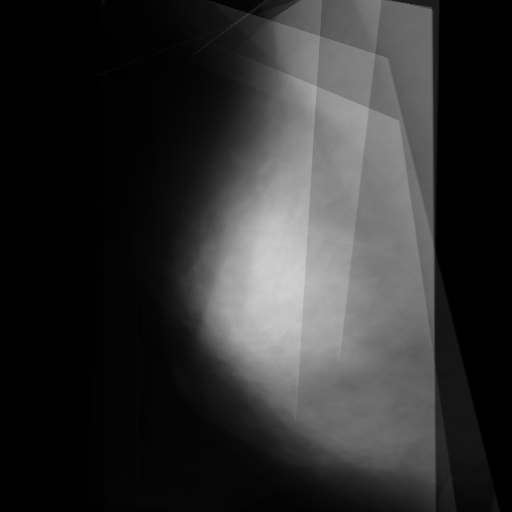
\includegraphics[width=\textwidth]{Appendix5/sample3/nonProb/20_scan.png}
      \caption{20 Non-Probabilistic Entropy iterations.}
      \label{fig:app-20-nonProb-sample3}
    \end{subfigure}
\end{figure}

\begin{table}[H]
  \begin{center}
    \pgfplotstabletypeset[col sep=comma,
        columns={Iteration,Entropy, Iteration, Entropy},columns/Entropy/.style={precision=6},
        every head row/.style={before row=\toprule,after row=\midrule},
        every last row/.style={after row=\bottomrule},
        display columns/0/.style={
            select equal part entry of={0}{2},
            string type,
            column name={Iteration (1/2)},
        },
        display columns/1/.style={
            select equal part entry of={0}{2},
            string type,
            column name={Entropy (1/2)},
        },
        display columns/2/.style={select equal part entry of={1}{2},string type}, column name={Iteration (2/2)},
        display columns/3/.style={select equal part entry of={1}{2},string type, column name={Entropy (2/2)}},
        ]{Appendix5/sample3/nonProb/nonProb.csv}
    \caption{Non-Probabilistic Entropy on Sample 3}
    \label{table:app-nonProb-entropy-3}
  \end{center}
\end{table}

\newpage \noindent \textbf{Sample 4 - BI-RADS IV}
Input image: Figure \ref{fig:app-sample4-input}

\begin{figure}[H]
    \centering
    \begin{subfigure}[t]{0.3\textwidth}
        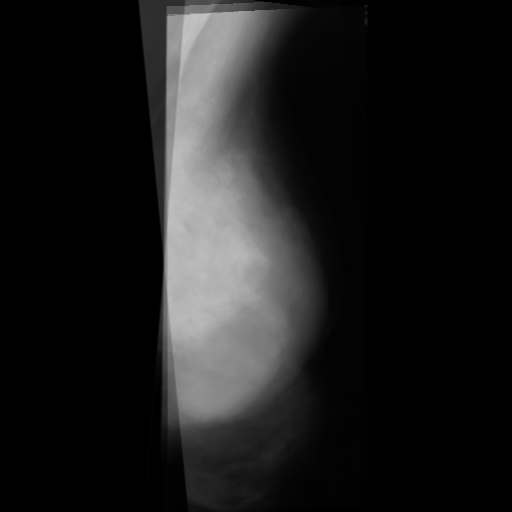
\includegraphics[width=\textwidth]{Appendix5/sample4/nonProb/scan_5.png}
        \caption{5 Non-Probabilistic Entropy iterations.}
        \label{fig:app-5-nonProb-sample4}
    \end{subfigure} \hfill
    ~ %add desired spacing between images, e. g. ~, \quad, \qquad, \hfill etc.
      %(or a blank line to force the subfigure onto a new line)
    \begin{subfigure}[t]{0.3\textwidth}
      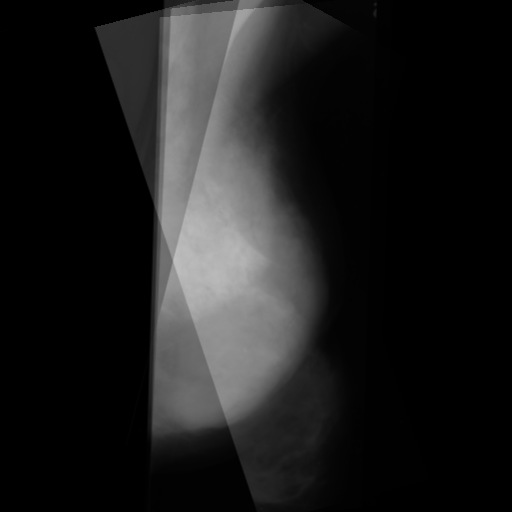
\includegraphics[width=\textwidth]{Appendix5/sample4/nonProb/scan_10.png}
      \caption{10 Non-Probabilistic Entropy iterations.}
      \label{fig:app-10-nonProb-sample4}
    \end{subfigure} \hfill
    \begin{subfigure}[t]{0.3\textwidth}
      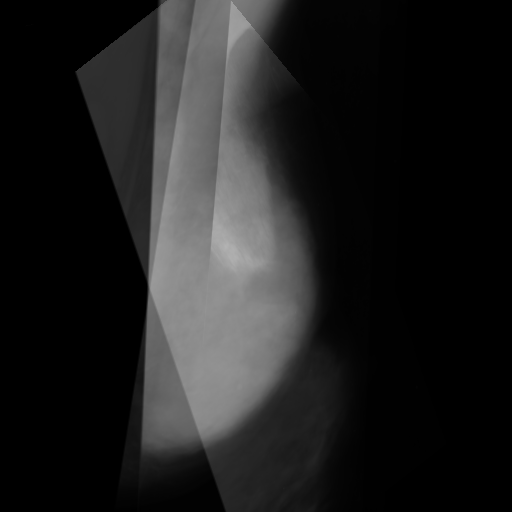
\includegraphics[width=\textwidth]{Appendix5/sample4/nonProb/20_scan.png}
      \caption{20 Non-Probabilistic Entropy iterations.}
      \label{fig:app-20-nonProb-sample4}
    \end{subfigure}
\end{figure}

\begin{table}[H]
  \begin{center}
    \pgfplotstabletypeset[col sep=comma,
        columns={Iteration,Entropy, Iteration, Entropy},columns/Entropy/.style={precision=6},
        every head row/.style={before row=\toprule,after row=\midrule},
        every last row/.style={after row=\bottomrule},
        display columns/0/.style={
            select equal part entry of={0}{2},
            string type,
            column name={Iteration (1/2)},
        },
        display columns/1/.style={
            select equal part entry of={0}{2},
            string type,
            column name={Entropy (1/2)},
        },
        display columns/2/.style={select equal part entry of={1}{2},string type}, column name={Iteration (2/2)},
        display columns/3/.style={select equal part entry of={1}{2},string type, column name={Entropy (2/2)}},
        ]{Appendix5/sample4/nonProb/nonProb.csv}
    \caption{Non-Probabilistic Entropy on Sample 4}
    \label{table:app-nonProb-entropy-4}
  \end{center}
\end{table}

\newpage
\section{Hybrid Entropy}

\noindent \textbf{Sample 1 - BI-RADS I}

Input image: Figure \ref{fig:app-sample1-input}

\begin{figure}[H]
    \centering
    \begin{subfigure}[t]{0.3\textwidth}
        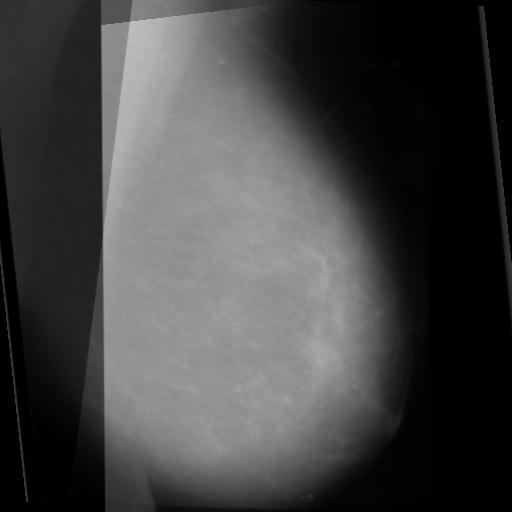
\includegraphics[width=\textwidth]{Appendix5/sample1/hybrid/hybrid-5.png}
        \caption{5 Hybrid Entropy iterations.}
        \label{fig:app-5-hybrid-sample1}
    \end{subfigure} \hfill
    ~ %add desired spacing between images, e. g. ~, \quad, \qquad, \hfill etc.
      %(or a blank line to force the subfigure onto a new line)
    \begin{subfigure}[t]{0.3\textwidth}
        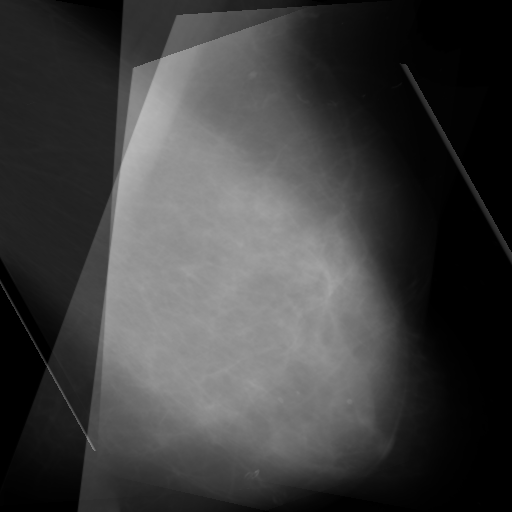
\includegraphics[width=\textwidth]{Appendix5/sample1/hybrid/hybrid-10.png}
        \caption{10 Hybrid Entropy iterations.}
        \label{fig:app-10-hybrid-sample1}
    \end{subfigure} \hfill
    \begin{subfigure}[t]{0.3\textwidth}
      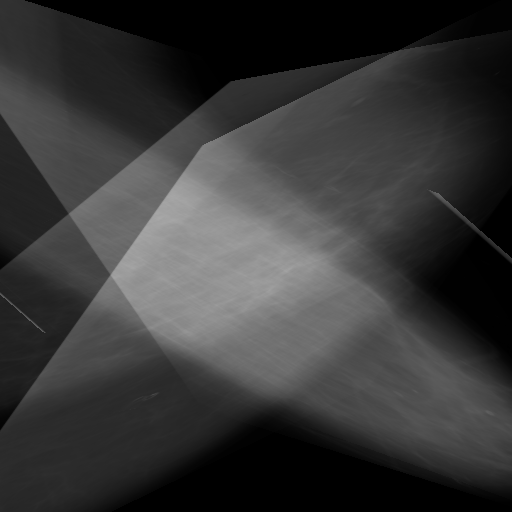
\includegraphics[width=\textwidth]{Appendix5/sample1/hybrid/hybrid20.png}
      \caption{20 Hybrid Entropy iterations.}
      \label{fig:app-20-hybrid-sample1}
    \end{subfigure}
\end{figure}

\begin{table}[H]
  \begin{center}
    \pgfplotstabletypeset[col sep=comma,
        columns={Iteration,Entropy, Iteration, Entropy},columns/Entropy/.style={precision=6},
        every head row/.style={before row=\toprule,after row=\midrule},
        every last row/.style={after row=\bottomrule},
        display columns/0/.style={
            select equal part entry of={0}{2},
            string type,
            column name={Iteration (1/2)},
        },
        display columns/1/.style={
            select equal part entry of={0}{2},
            string type,
            column name={Entropy (1/2)},
        },
        display columns/2/.style={select equal part entry of={1}{2},string type}, column name={Iteration (2/2)},
        display columns/3/.style={select equal part entry of={1}{2},string type, column name={Entropy (2/2)}},
        ]{Appendix5/sample1/hybrid/hybrid20.csv}
    \caption{Hybrid Entropy on Sample 1}
    \label{table:app-hybrid-entropy-1}
  \end{center}
\end{table}

\newpage \noindent \textbf{Sample 2 - BI-RADS II}

Input image: Figure \ref{fig:app-sample2-input}

\begin{figure}[H]
    \centering
    \begin{subfigure}[t]{0.3\textwidth}
        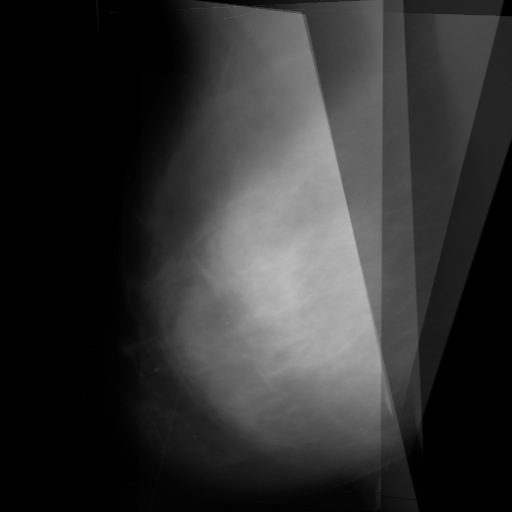
\includegraphics[width=\textwidth]{Appendix5/sample2/hybrid/5_hybrid.png}
        \caption{5 Hybrid Entropy iterations.}
        \label{fig:app-5-hybrid-sample2}
    \end{subfigure} \hfill
    ~ %add desired spacing between images, e. g. ~, \quad, \qquad, \hfill etc.
      %(or a blank line to force the subfigure onto a new line)
    \begin{subfigure}[t]{0.3\textwidth}
        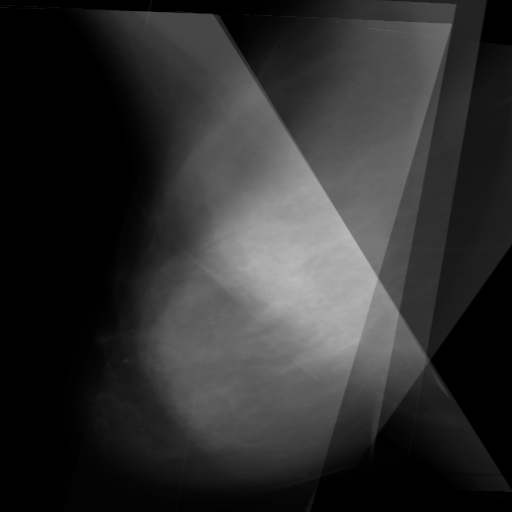
\includegraphics[width=\textwidth]{Appendix5/sample2/hybrid/10_hybrid.png}
        \caption{10 Hybrid Entropy iterations.}
        \label{fig:app-10-hybrid-sample2}
    \end{subfigure} \hfill
    \begin{subfigure}[t]{0.3\textwidth}
      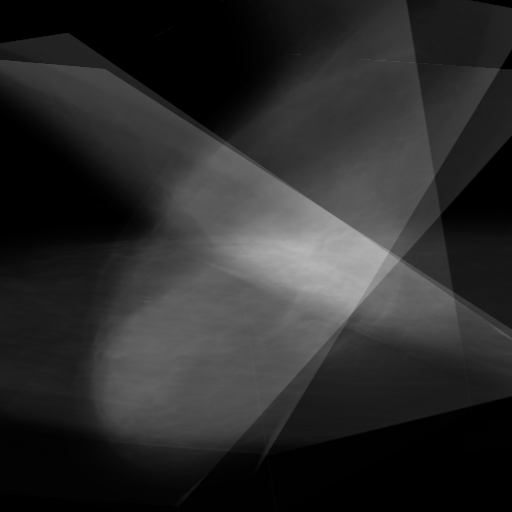
\includegraphics[width=\textwidth]{Appendix5/sample2/hybrid/20_hybrid.png}
      \caption{20 Hybrid Entropy iterations.}
      \label{fig:app-20-hybrid-sample2}
    \end{subfigure}
\end{figure}

\begin{table}[H]
  \begin{center}
    \pgfplotstabletypeset[col sep=comma,
        columns={Iteration,Entropy, Iteration, Entropy},columns/Entropy/.style={precision=6},
        every head row/.style={before row=\toprule,after row=\midrule},
        every last row/.style={after row=\bottomrule},
        display columns/0/.style={
            select equal part entry of={0}{2},
            string type,
            column name={Iteration (1/2)},
        },
        display columns/1/.style={
            select equal part entry of={0}{2},
            string type,
            column name={Entropy (1/2)},
        },
        display columns/2/.style={select equal part entry of={1}{2},string type}, column name={Iteration (2/2)},
        display columns/3/.style={select equal part entry of={1}{2},string type, column name={Entropy (2/2)}},
        ]{Appendix5/sample2/hybrid/hybrid.csv}
    \caption{Hybrid Entropy on Sample 2}
    \label{table:app-hybrid-entropy-2}
  \end{center}
\end{table}

\newpage
\noindent \textbf{Sample 3 - BI-RADS III}

Input image: Figure \ref{fig:app-sample3-input}

\begin{figure}[H]
    \centering
    \begin{subfigure}[t]{0.3\textwidth}
        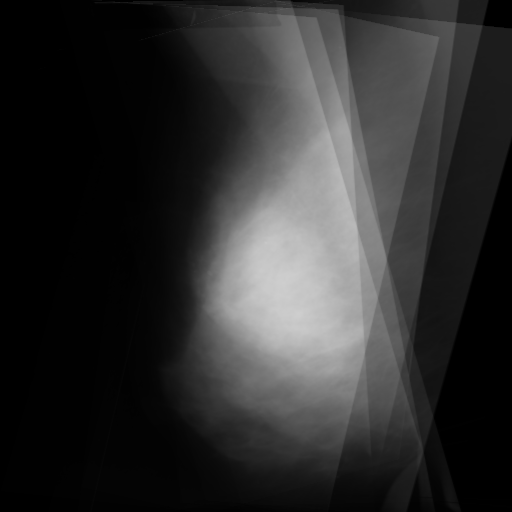
\includegraphics[width=\textwidth]{Appendix5/sample3/hybrid/5_hybrid.png}
        \caption{5 Hybrid Entropy iterations.}
        \label{fig:app-5-hybrid-sample3}
    \end{subfigure} \hfill
    ~ %add desired spacing between images, e. g. ~, \quad, \qquad, \hfill etc.
      %(or a blank line to force the subfigure onto a new line)
    \begin{subfigure}[t]{0.3\textwidth}
        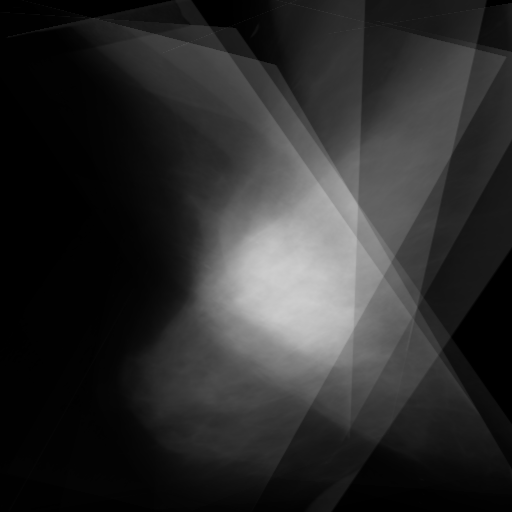
\includegraphics[width=\textwidth]{Appendix5/sample3/hybrid/10_hybrid.png}
        \caption{10 Hybrid Entropy iterations.}
        \label{fig:app-10-hybrid-sample3}
    \end{subfigure} \hfill
    \begin{subfigure}[t]{0.3\textwidth}
      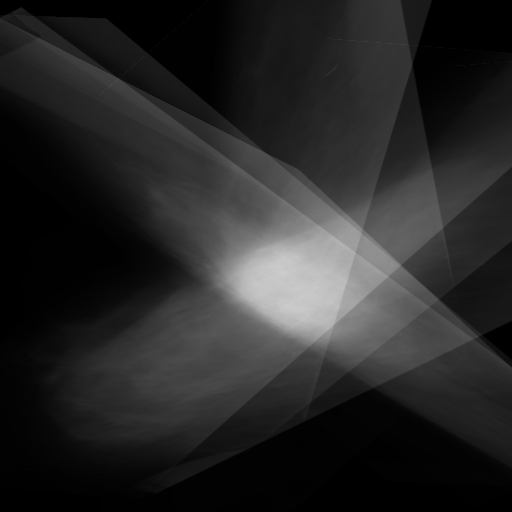
\includegraphics[width=\textwidth]{Appendix5/sample3/hybrid/20_hybrid.png}
      \caption{20 Hybrid Entropy iterations.}
      \label{fig:app-20-hybrid-sample3}
    \end{subfigure}
\end{figure}

\begin{table}[H]
  \begin{center}
    \pgfplotstabletypeset[col sep=comma,
        columns={Iteration,Entropy, Iteration, Entropy},columns/Entropy/.style={precision=6},
        every head row/.style={before row=\toprule,after row=\midrule},
        every last row/.style={after row=\bottomrule},
        display columns/0/.style={
            select equal part entry of={0}{2},
            string type,
            column name={Iteration (1/2)},
        },
        display columns/1/.style={
            select equal part entry of={0}{2},
            string type,
            column name={Entropy (1/2)},
        },
        display columns/2/.style={select equal part entry of={1}{2},string type}, column name={Iteration (2/2)},
        display columns/3/.style={select equal part entry of={1}{2},string type, column name={Entropy (2/2)}},
        ]{Appendix5/sample3/hybrid/hybrid.csv}
    \caption{Hybrid Entropy on Sample 3}
    \label{table:app-hybrid-entropy-3}
  \end{center}
\end{table}

\newpage \noindent \textbf{Sample 4 - BI-RADS IV}

Input image: Figure \ref{fig:app-sample4-input}

\begin{figure}[H]
    \centering
    \begin{subfigure}[t]{0.3\textwidth}
        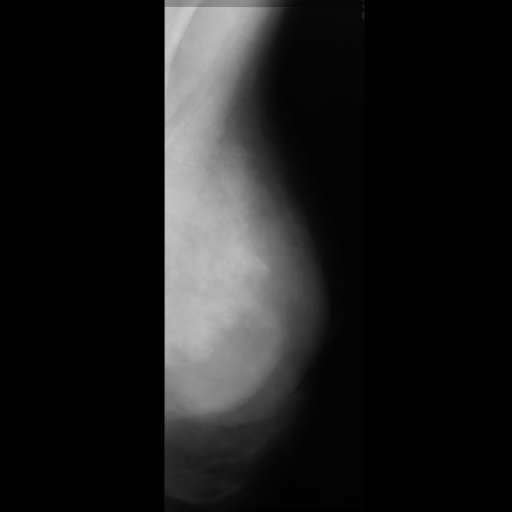
\includegraphics[width=\textwidth]{Appendix5/sample4/hybrid/hybrid_5.png}
        \caption{5 Hybrid Entropy iterations.}
        \label{fig:app-5-hybrid-sample4}
    \end{subfigure} \hfill
    ~ %add desired spacing between images, e. g. ~, \quad, \qquad, \hfill etc.
      %(or a blank line to force the subfigure onto a new line)
    \begin{subfigure}[t]{0.3\textwidth}
        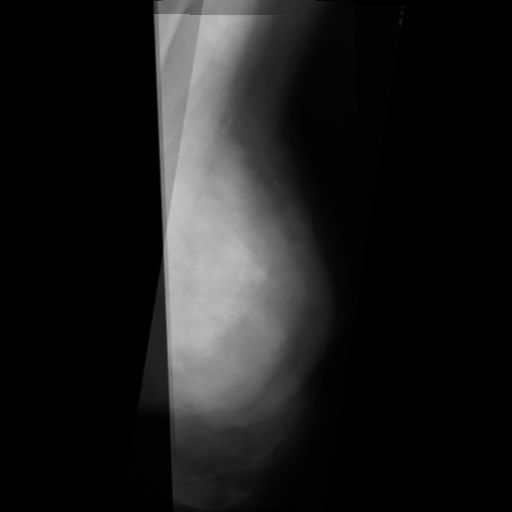
\includegraphics[width=\textwidth]{Appendix5/sample4/hybrid/hybrid_10.png}
        \caption{10 Hybrid Entropy iterations.}
        \label{fig:app-10-hybrid-sample4}
    \end{subfigure} \hfill
    \begin{subfigure}[t]{0.3\textwidth}
      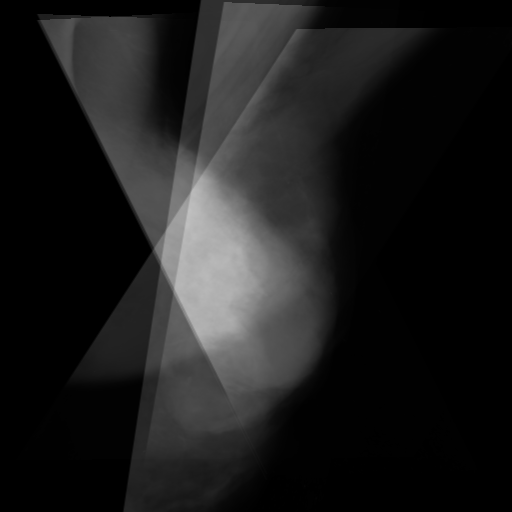
\includegraphics[width=\textwidth]{Appendix5/sample4/hybrid/hybrid_20.png}
      \caption{20 Hybrid Entropy iterations.}
      \label{fig:app-20-hybrid-sample4}
    \end{subfigure}
\end{figure}

\begin{table}[H]
  \begin{center}
    \pgfplotstabletypeset[col sep=comma,
        columns={Iteration,Entropy, Iteration, Entropy},columns/Entropy/.style={precision=6},
        every head row/.style={before row=\toprule,after row=\midrule},
        every last row/.style={after row=\bottomrule},
        display columns/0/.style={
            select equal part entry of={0}{2},
            string type,
            column name={Iteration (1/2)},
        },
        display columns/1/.style={
            select equal part entry of={0}{2},
            string type,
            column name={Entropy (1/2)},
        },
        display columns/2/.style={select equal part entry of={1}{2},string type}, column name={Iteration (2/2)},
        display columns/3/.style={select equal part entry of={1}{2},string type, column name={Entropy (2/2)}},
        ]{Appendix5/sample4/hybrid/hybrid.csv}
    \caption{Hybrid Entropy on Sample 4}
    \label{table:app-hybrid-entropy-4}
  \end{center}
\end{table}

%TC:endignore
